\documentclass{weekprobleem}
\usepackage[utf8]{inputenc}
\usepackage{gensymb}
\usepackage{graphicx}
\usepackage{wrapfig}

\usepackage[LGR,T1]{fontenc}
\usepackage{textalpha}
\newcommand{\textgreek}[1]{\begingroup\fontencoding{LGR}\selectfont#1\endgroup}

\begin{document}
\weekprobleem{2017}{C}{Creatieve weekproblemen: scheepvaart}

\begin{wrapfigure}[9]{o}[2cm]{6cm}
	\vspace{-6mm}
	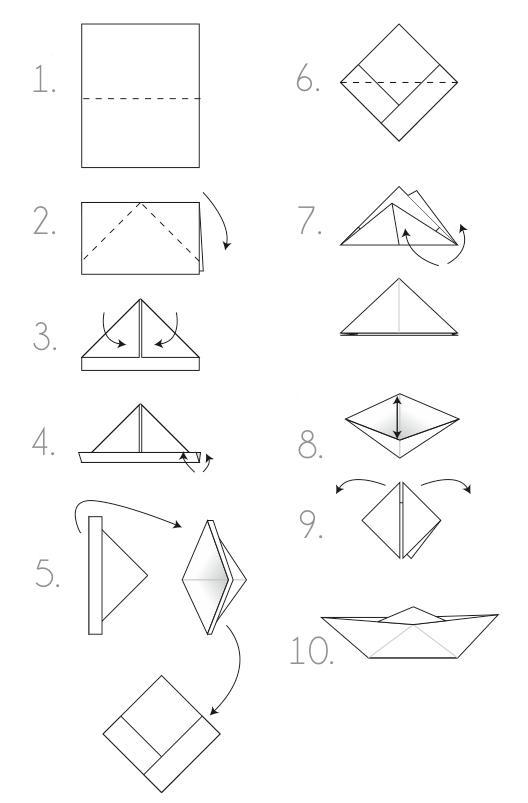
\includegraphics[width=6cm]{origami-boot}
	\vspace{-0mm}
\end{wrapfigure}

Dit jaar hebben de creatieve weekproblemen het thema scheepvaart.

\section*{Vouw een boot}

Vrijwel iedereen weet hoe je van een A5'je een bootje kunt vouwen, maar bootje dat je krijgt is op groter formaat een beetje saai.

De opdracht: neem een vel A3-papier en vouw een bootje, en probeer er zo veel mogelijk details in te origamiën.
Denk hierbij bijvoorbeeld de hut van de kapitein, een zeemeerminnenboegbeeld, of een radar-antenne.

Let op: zoals gebruikelijk bij origami zijn de bouwwerken gemaakt van één stuk papier, en zonder gebruik te maken van een schaar of plakband.
{\tiny (Goed verstoppen dus!)}


\section*{Maak een sterrenbeeld}

\begin{figure}
	\centering
	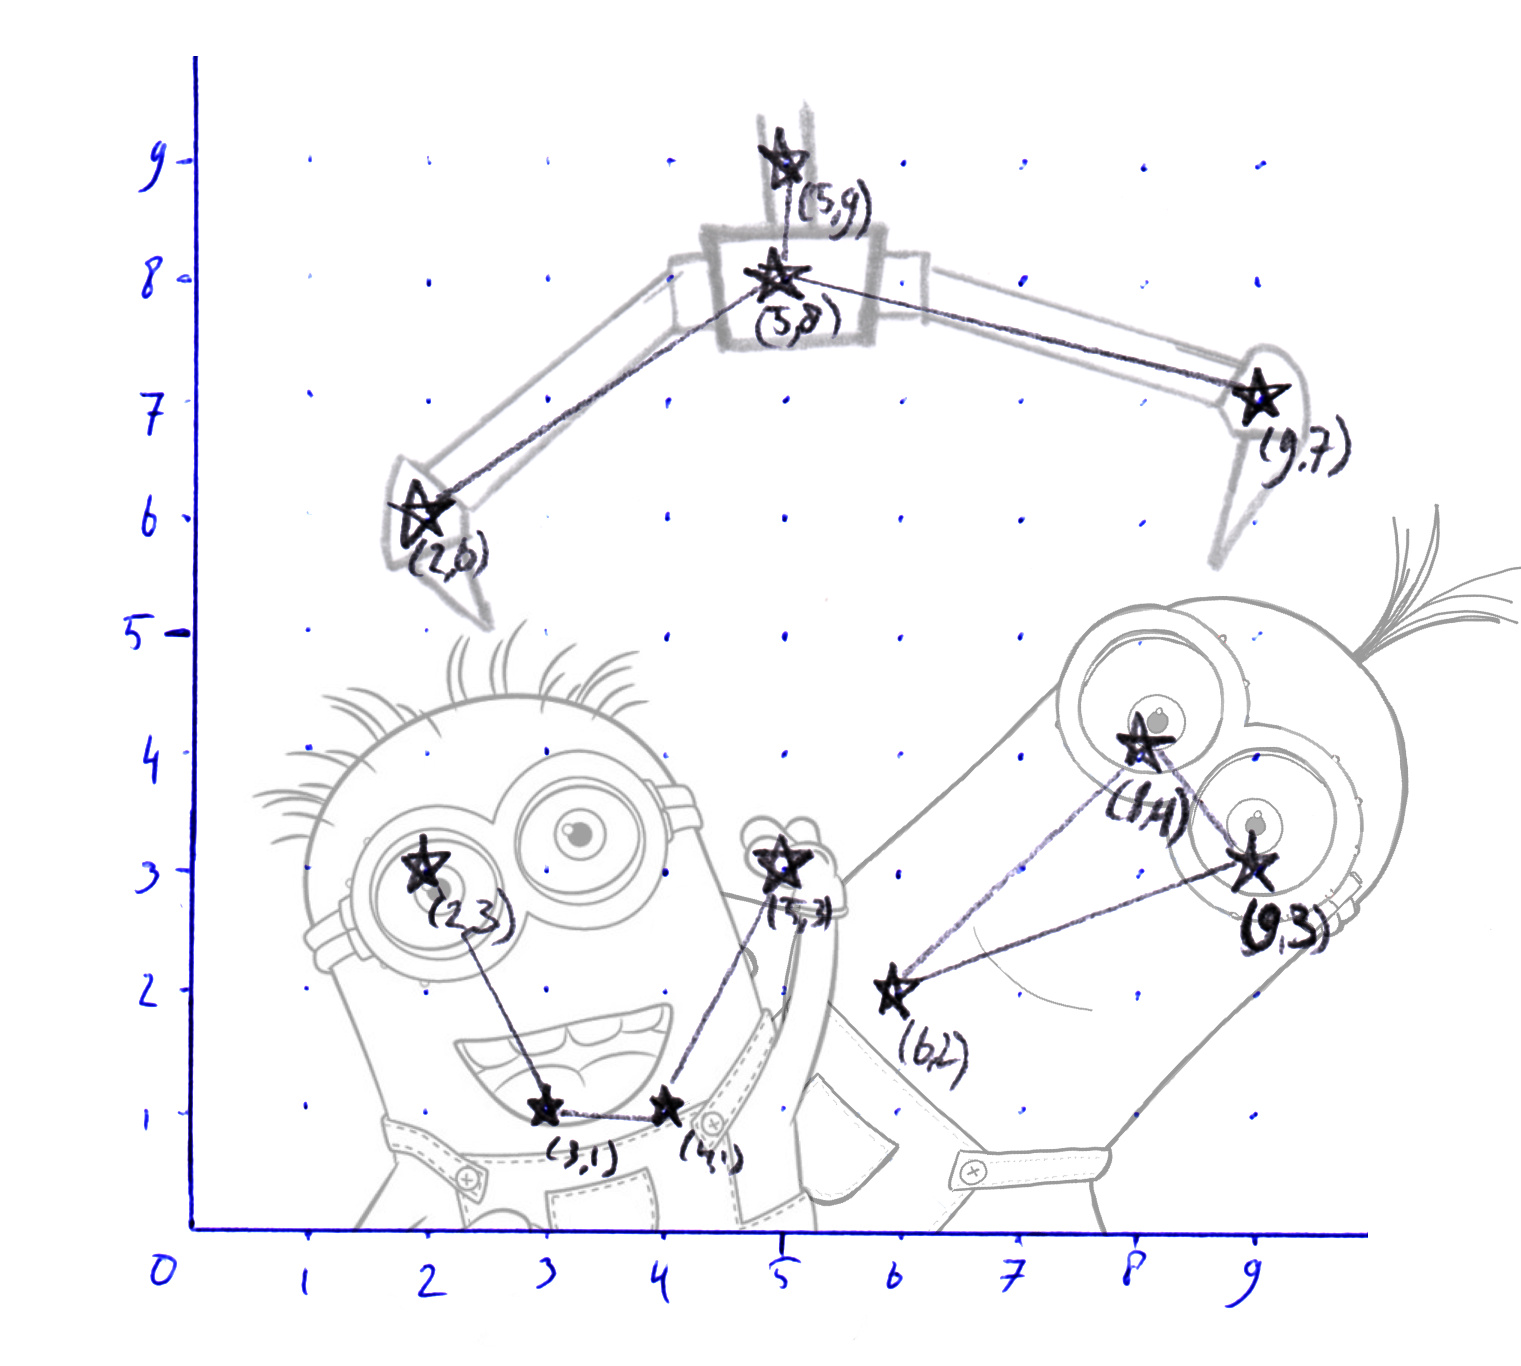
\includegraphics[width=10cm]{pi}
	\caption{\small{In dit voorbeeld hebben we $\pi$ tot een sterrenbeeld gemaakt door de volgende punten op ruitjespapier te tekenen: $\{(3,1), (4,1), (5,9), \ldots (8,4), (6,2)\}$. Het sterrenbeeld heet ``Twee Minions in een Hijskraanspelletje op de Kermis.'' De oude Grieken zagen dit sterrenbeeld bij besteding van 15 Drachmen of meer in de plaatselijke \textgreek{Albertos \<Einos}.}}
\end{figure}
Tegenwoordig heeft bijna iedereen een GPS-antenne in zijn of haar broekzak, maar honderd jaar geleden ging dat héél anders: schepen die de oceanen afstruinden moesten navigeren op de sterren.
Om de scheepvaarders wat te helpen ga je een nieuw sterrenbeeld maken.

Neem je favoriete irrationele getal ($\pi$, $e$, $\sqrt{2}$, etc.), en verzin een manier om van de decimalen een sterrenbeeld van te maken.
Je kunt bijvoorbeeld de decimalen in een coördinatensysteem tekenen en er lijntjes tussen trekken, of je eigen systeem verzinnen zoals "$3$ cm vooruit, $141{\degree}$ naar rechts, $5$ cm vooruit, $92{\degree}$ naar links, $6$ cm vooruit, enzovoort".

Wat beeldt je lijnentekening uit?\\
Wat is het mythologische verhaal achter jouw sterrenbeeld?\\
Welke ster is het belangrijkst voor de scheepvaarders? Waarom? Wijst deze ster bijvoorbeeld altijd naar de dichtstbijzijnde McDonalds?


\section*{Gestrand!}

Helaas, het sterrenbeeld van hierboven bleek toch niet betrouwbaar genoeg om de weg te vinden, en de boot van nog eerder was niet stevig genoeg om een botsing met een klein eiland te weerstaan. Je bent gestrand!

Als je vier getallen mocht meenemen naar een onbewoond eiland om je gezelschap te houden, welke zou je dan kiezen? Waarom?\\
Schrijf een verhaal over de avonturen die jullie met zijn vijven beleven.

\end{document} 
